\chapter{SuPerHomog\'{e}n\'{e}isation Factors}
\label{chap:sph}

The results in Chapter~\ref{chap:biases} demonstrated that using the ``true'' flux spectrum from Monte Carlo to perform energy condensation and spatial homogenization will not necessarily result in accurate deterministic multi-group calculations. Large systematic biases in the eigenvalue were observed for simple heterogeneous benchmark models. In Section~\ref{sec:chap5-diagnosis} it was shown that the bias largely derives from errors in the multi-group reaction rates in the large thermal U-238 capture resonances. These results indicate that one or more of the approximations made in multi-group transport theory are invalidated in heterogeneous geometries and prevent an appropriate treatment of spatial self-shielding at the fuel/moderator interface in \ac{PWR} geometries.

%, and that the errors systematically vary in space within the fuel.

%, and these biases were highly dependent on the energy group structure and spatial discretization used in the multi-group deterministic calculation.

Chap.~\ref{chap:mgxs} discussed approximations made in multi-group theory to simplify the neutron transport equation in angle, energy and space. Many of these approximations were quantitatively studied in Chap.~\ref{chap:biases} -- including energy group structure, spatial discretization mesh, and isotropic scattering -- yet it was demonstrated that none of these led to the eigenvalue bias. This chapter investigates the flux separability approximation as the dominant factor contributing to the eigenvalue bias.

Sec~\ref{sec:chap6-angular-mgxs} reviews some recent work by by Gibson~\cite{gibson2016thesis} to quantify the approximation error resolved with angular-dependent \ac{MGXS}, which closely mirrors the trends observed in Chap.~\ref{chap:biases}. The historical \ac{SPH} factor concept is introduced in the context of angular-dependent \ac{MGXS} in Sec.~\ref{sec:chap6-sph}, and \ac{SPH} factors are applied to simple heterogeneous benchmarks and the results analyzed in Sec.~\ref{sec:chap6-sph}. Finally, this chapter concludes with a summary of the shortcomings of the \ac{SPH} approach and the need for new methods to account for the angular dependence in \ac{MGXS}.

%first paragraph: motivate problem
%-mention bias from nelson/yoshikoka 


%%%%%%%%%%%%%%%%%%%%%%%%%%%%%%%%%%%%%%%%%%%%%%%%%%%%%%%%%%%%%%%%%%%%%%%%%%%%%%%
\section{Angular-Dependent MGXS}
\label{sec:chap6-angular-mgxs}

The flux separability approximation introduced in Sec.~\ref{subsec:chap2-angle} led to the use of the scalar rather than the angular flux to condense the total cross section in energy. The mathematically proper treatment would instead use the angular flux to condense the total \ac{MGXS} in angle, energy and space, resulting in angular-dependent total \ac{MGXS}. Flux separability is commonly used since conventional \ac{MGXS} generation schemes are generally incapable of approximating the angular dependence of the flux. Nevertheless, flux separability is an approximation which may lead to non-trivial errors in downstream multi-group calculations, such as the eigenvalue bias observed in Chap.~\ref{chap:biases}. 

The flux separability approximation will necessarily hold in infinite homogeneous media -- such as that considered in Sec.~\ref{subsec:chap5-inf-medium} -- since the flux does not vary in angle or space. However, the flux may vary greatly by angle in a heterogeneous geometry with significant spatial self-shielding. For example, consider the flux from two different directions impinged upon the \ac{FSR} for one radial ring and angular sector in a fuel pin in Fig.~\ref{fig:chap6-incoming-outgoing}. The flux entering from the moderator will be unshielded and will likely be quite similar to the $\nicefrac{1}{E}$ asymptotic spectrum. In contrast, the flux which traverses the fuel pin will be signficantly depressed in the resonant groups. As a result, the reaction rates for the incoming flux will be greater than those for the outgoing flux in resonant groups, which would be reflected in angular-dependent total \ac{MGXS}.

\begin{figure}[h]
  \centering
  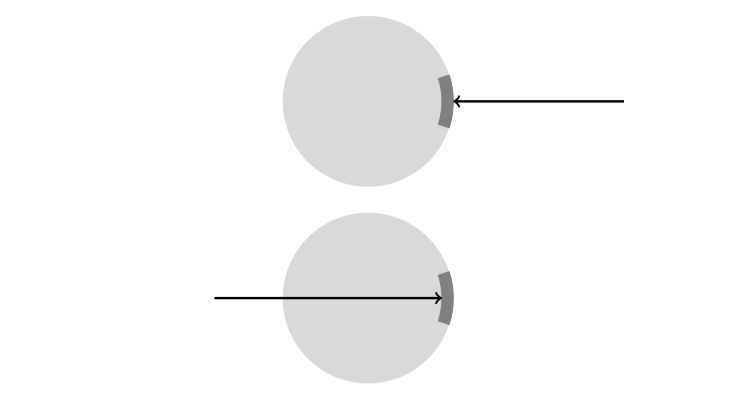
\includegraphics[width=\linewidth]{figures/sph/incoming-outgoing}
  \caption[Angular flux impinged on an FSR]{Angular flux impinged on an FSR from the moderator (top) and after traversing the fuel (bottom). \textit{Image courtesy of N. Gibson~\cite{gibson2016thesis}.}}
\label{fig:chap6-incoming-outgoing}
\end{figure}

A recent PhD thesis by Gibson~\cite{gibson2016thesis} studied the impact of using angular-dependent total \ac{MGXS} on multi-group calculations to avoid the flux separability approximation. Gibson was motivated by his observation of reaction rate errors similar to those discovered in Sec.~\ref{sec:chap5-diagnosis}. In particular, he solved for the reference ultra-fine flux for a 2D \ac{PWR} fuel pin given a fixed source. The reference scalar flux was used to condense the continuous energy total cross sections to 69-group \ac{MGXS}, which were employed in a second fixed source transport calculation. The reaction rates computed from the ultra-fine and 69-group scalar fluxes differed by up to 1\% for low-lying energy groups with large U-238 capture resonances, with an error profile in energy similar to that in Fig.~\ref{fig:chap5-rel-err-energy}. Gibson's results indicated that an improper treatment of self-shielding effects in heterogeneous geometries may lead to errors in resonant groups even when the exact scalar flux is used to collapse cross sections in energy and space.

Gibson further investigated this issue by using the reference ultra-fine angular flux to compute angular-dependent \ac{MGXS}. Some examples of the angular-dependent capture \ac{MGXS} generated for two different \ac{FSR}s shaded in dark gray are shown in Fig.~\ref{fig:chap6-batman-plots}. The \ac{MGXS} in the \ac{FSR} at the fuel/moderator interface in Fig.~\ref{fig:chap6-batman-plots-a} ranges from less than 5 to more than 30 barns for angles entering and leaving the fuel pin. The peaks near 60$^{\circ}$ and 120$^{\circ}$ are due to extra moderation experienced by neutrons streaming through the infinite rectilinear fuel pin lattice at those angles. The \ac{MGXS} in \ac{FSR}s in the interior of the fuel pin, such as the one shown in Fig.~\ref{fig:chap6-batman-plots-b}, exhibit similar but less prominent properties since the flux is shielded in all directions.

\begin{figure}[h]
\begin{subfigure}{.5\textwidth}
  \centering
  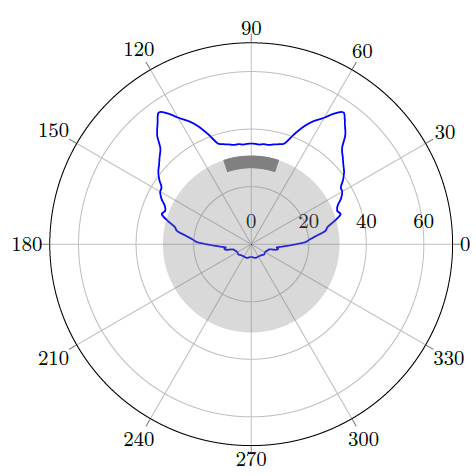
\includegraphics[width=\linewidth]{figures/sph/batman-1}
  \caption{}
  \label{fig:chap6-batman-plots-a}
\end{subfigure}
\begin{subfigure}{.5\textwidth}
  \centering
  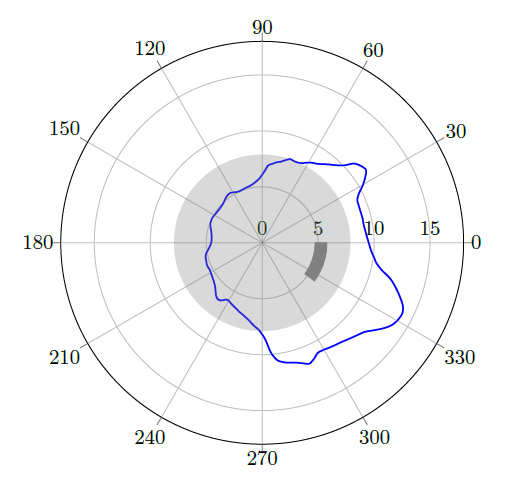
\includegraphics[width=\linewidth]{figures/sph/batman-2}
  \caption{}
  \label{fig:chap6-batman-plots-b}
\end{subfigure}
\caption[Angular-dependent capture MGXS]{Angular-dependent capture \ac{MGXS} as a function of incoming azimuthal angle for two different \ac{FSR}s for the 6.67 eV resonance group. The radial axis is given in units of barns and the azimuthal axis in units of degrees. \textit{Image courtesy of N. Gibson~\cite{gibson2016thesis}.}}
\label{fig:chap6-batman-plots}
\end{figure}

Gibson proceeded to show that the angular-dependent total \ac{MGXS} eliminated the reaction rate errors observed with scalar flux-weighted \ac{MGXS}. His analysis highlighted the tight coupling between angular dependence and the spatial discretization. Notably, the reaction rate errors were reduced by an order of magnitude only when angular-dependent \ac{MGXS} were paired with a fine \ac{FSR} spatial discretization. This can be explained by the fact that the angular variation of the volume-integrated flux is diminished as the \ac{FSR} mesh is coarsened. Thus, the spatial self-shielding effects at the fuel/moderator interface cannot be captured by angular-dependent total \ac{MGXS} if the \ac{FSR} discretization is unable to distinguish between neutrons entering/leaving the fuel pin.

Although angular-dependent total \ac{MGXS} is the most direct solution to eliminate the flux separability approximation, it is not a desirable approach for a number of reasons. Angular-dependent \ac{MGXS} would significantly increase the memory footprint for \ac{MGXS} libraries, and be complicated to accommodate in multi-group methods. Furthermore, angular-dependent \ac{MGXS} is not attractive for \ac{MC}-based \ac{MGXS} generation since many more particle histories would be required to converge the \ac{MGXS} in each discrete angular tally bin. The Consistent-P approximation~\cite{bell1967transport} is an alternative method that embeds the angular dependence of the total \ac{MGXS} within the angular expansion of the scattering kernel (Eqn.~\ref{eqn:chap2-transport-ce-2}) while retaining an angular independent total \ac{MGXS}. Although the Consistent-P approximation is one viable approach used in many transport codes, it was not evaluated here since anisotropic scattering was not implemented in OpenMOC at the time of this writing. A third method known SuPerHomog\'{e}n\'{e}isation factors was discussed in this context by Gibson, who employed them to reduce heterogeneous resonant reaction rate errors (albeit to a lesser extent than he achieved with angular-depenent total \ac{MGXS}). \ac{SPH} factors are a relatively simple-to-implement method which do not require an anisotropic scattering kernel implementation. For this reason, the \ac{SPH} factor scheme was evaluated in OpenMOC as discussed in the following sections.

%-Nelson's 1D slab plot(s)?


%%%%%%%%%%%%%%%%%%%%%%%%%%%%%%%%%%%%%%%%%%%%%%%%%%%%%%%%%%%%%%%%%%%%%%%%%%%%%%%
\section{SuPerHomog\'{e}n\'{e}isation Factors}
\label{sec:chap6-sph}

first paragraph: motivate following section
-alternative approach is SPH
-forces neutron balance
-recall nate's thesis
-intro following sections

% requires a fixed source solver and a reference source, both of which are known from \ac{MC} tallies with 

%Although \ac{SPH} factors were introduced more than two decades ago, to this author's knowledge

%%%%%%%%%%%%%%%%%%%%%
\subsection{Overview}
\label{subsec:chap6-sph-overview}

first paragraph: SPH factors
-history w/ H\'{e}bert~\cite{hebert1993consistent}\cite{hebert2005ribon}
-recall nate's thesis
-high-level overview
-traditionally used in diffusion applications
-used to fix errors in energy condensation and spatial homogenization
  -this could include all kinds of errors -- not really discussed in the literature

second paragraph: walk through eqns
-start w/ spatially-homogenized and energy condensed transport eqn in Eqn.~\ref{eqn:chap2-transport-mg-5}
-walk through eqns to preserve neutron balance

-transport eqn with arbitrary fixed source and 

\begin{dmath}
\label{eqn:chap6-sph-transport-eqn}
\mathbf{\Omega} \cdot \nabla \psi_{g}(\mathbf{r},\mathbf{\Omega}) + \mu_{k,g}\Sigma_{t,k,g}\psi_{g}(\mathbf{r},\mathbf{\Omega}) = Q_{k,g}(\mathbf{\Omega})
\end{dmath}

-this equation is solved for all groups simultaneously with fixed source solver in OpenMOC

-should there be another section on SPH with Monte Carlo? This would highlight that the source is computed
-note that the source is computed using the reference Monte Carlo flux:
-the source is computed as a pre-processing step from the reference Monte Carlo flux
-the source never changes during the iteration

\begin{dmath}
\label{eqn:chap6-sph-source}
Q_{k,g}(\mathbf{\Omega}) = \frac{1}{4\pi} \sum_{g'=1}^{G} \Sigma_{s,k,g' \rightarrow g}\phi_{k,g'}^{MC} + \frac{\chi_{k,g}}{4\pi k_{eff}}\sum_{g'=1}^{G} \nu\Sigma_{f,k,g'}\phi_{k,g'}
\end{dmath}

-general SPH factor
-make these equations independent of iteration number - i.e., these are the equations we want
-use a hat above SPH factor below 
-this section should just pose the problem - need to find the factors that preserve reaction rates

%%%%%%%%%%%%%%%%%%%%%
\subsection{Algorithm}
\label{subsec:chap6-sph-overview}

-mention that the MC source calculation is not trivial
-tallies are volume-integrated in OpenMC, while values are volume-averaged in OpenMOC
-must compute volume-averaged sources for OpenMOC
  -must be averaged with the volume computed by OpenMOC from track lengths!!!

-the SPH factor is then necessarily defined as the ratio of computed to reference fluxes:

\begin{dmath}
\label{eqn:chap6-sph-transport-eqn-iterate}
\mathbf{\Omega} \cdot \nabla \psi_{g}^{(n)}(\mathbf{r},\mathbf{\Omega}) + \hat{\mu}_{k,g}\Sigma_{t,k,g}\psi_{g}^{(n)}(\mathbf{r},\mathbf{\Omega}) = Q_{k,g}(\mathbf{\Omega})
\end{dmath}

\begin{dmath}
\label{eqn:chap6-sph-initial}
\hat{\mu}_{k,g}^{(0)} = 1
\end{dmath}

\begin{equation}
\label{eqn:chap6-sph-update}
\hat{\mu}_{k,g}^{(n)} = \frac{\phi_{k,g}^{MC}}{\phi_{k,g}^{(n)}}
\end{equation}

-update the total MGXS
-note that although sigs and nusigf are updated, this does not impact fixed source calculations for SPH iteration and only affects eigenvalue calculations with the SPH-corrected MGXS

\begin{dmath}
\label{eqn:chap6-sph-update-sigt}
\Sigma_{t,k,g}^{(n)} = \hat{\mu}_{k,g}^{(n-1)}\Sigma_{t,k,g}^{(0)}
\end{dmath}

\begin{dmath}
\label{eqn:chap6-sph-update-sigs}
\Sigma_{s,k,g'\rightarrow g}^{(n)} = \hat{\mu}_{k,g}^{(n-1)}\Sigma_{s,k,g'\rightarrow g}^{(0)}
\end{dmath}

\begin{dmath}
\label{eqn:chap6-sph-update-nusigf}
\nu\Sigma_{f,k,g}^{(n)} = \hat{\mu}_{k,g}^{(n-1)}\nu\Sigma_{f,k,g}^{(0)}
\end{dmath}

-similarly, the flux can be recovered as:

\begin{dmath}
\label{eqn:chap6-sph-update-angular-flux}
\psi_{k,g} = \hat{\mu}_{k,g}^{(n-1)}\psi_{k,g}
\end{dmath}

\begin{dmath}
\label{eqn:chap6-sph-update-scalar-flux}
\phi_{k,g} = \hat{\mu}_{k,g}^{(n-1)}\phi_{k,g}
\end{dmath}

-SPH factor residual used to determine convergence
-a criterion of 1E-6 is typically used?

\begin{dmath}
\label{eqn:chap6-sph-residual}
res = \max_{k,g} \left|\frac{\hat{\mu}_{k,g}^{(n)} - \hat{\mu}_{k,g}^{(n-1)}}{\hat{\mu}_{k,g}^{(n-1)}}\right|
\end{dmath}

third paragraph: intro algorithm
-walk through the algorithm
-mention that typically done on a group-wise basis
-can be done with all group simultaneously
-mention that this is not trivial to implement on an unstructured \ac{CG} mesh!!!

\begin{algorithm}[h]
\caption{SPH Factor Algorithm}
\label{alg:chap6-sph}
\begin{algorithmic}[1]
  \State Initialize $\Sigma_{t,k,g}^{(0)}$, $\Sigma_{s,k,g'\rightarrow g}^{(0)}$, $\nu\Sigma_{f,k,g}^{(0)}$, and $\chi_{k,g}^{(0)}$ from MC tallies \Comment{Tab.~\ref{table:chap3-tally-types}}
  \State Compute $Q_{k,g}$ from MC flux and \ac{MGXS} \Comment{Eqn.~\ref{eqn:chap6-sph-source}}
  \State Initialize $\hat{\mu}_{k,g}^{(0)}$ to unity
  \While{SPH factors are not converged}
    \State Update $\Sigma_{t,k,g}$ with \ac{SPH} factors \Comment{Eqn.~\ref{eqn:chap6-sph-update-sigt}}
    \State Solve fixed source transport problem\footnotemark \Comment{Eqn.~\ref{eqn:chap6-sph-transport-eqn}}
    \State Compute new \ac{SPH} factors \Comment{Eqn.~\ref{eqn:chap6-sph-update}}
  \EndWhile
  \State Compute final \ac{MGXS} with \ac{SPH} factors \Comment{Eqn.~\Crefrange{eqn:chap6-sph-update-sigt}{eqn:chap6-sph-update-nusigf}}
\end{algorithmic}
\end{algorithm}

\footnotetext{A series of $G$ independent fixed source problems may be solved for each of the $G$ groups. Alternatively, a single fixed source problem may simultaneously solve for all $G$ groups, as is done in OpenMOC.}

ALGORITHM HERE (GROUP-BY-GROUP)\\

fourth paragraph: summary
-fudge factors that attempt to preserve reaction rates


%%%%%%%%%%%%%%%%%%%%%%%%%%%%%%%%%%%%%%
\subsection{Implementation in OpenMOC}
\label{subsec:chap6-sph-openmoc}

first paragraph: in openmoc.materialize
-implementation of SPH factors in openmoc
-custom for openmc.mgxs Library objects

second paragraph: intro algorithm
-walk through the algorithm

ALGORITHM HERE (SIMULTANEOUS GROUPS)\\


The results in Chapter~\ref{chap:biases} demonstrated systematic biases between continuous energy Monte Carlo and deterministic multi-group simulations of simple heterogeneous benchmark models. In Section~\ref{sec:chap5-diagnosis} it was shown that these biases largely derive from errors in the multi-group fluxes/reaction rates in the large thermal U-238 capture resonances. 

-sentence wrapping this paragraph up - talk about spatial self-shielding and segue

These results closely mirror observations by Gibson~\cite{gibson2016thesis} which quantified the errors fundamental to the total 


%%%%%%%%%%%%%%%%%%%%%%%%%%%%%%%%%%%%%%%%%%%%%%%%%%%%%%%%%%%%%%%%%%%%%%%%%%%%%%%
\section{Case Studies}
\label{sec:chap6-sph-case-studies}

first paragraph: intro case studies
-SPH applied to heterogeneous benchmarks from Chap. 5
-itemize covergence criterion
-fixed source criterion in openmoc
-fission source criterion in openmoc
-identify the metrics that will be presented in what follows:
  -reduction in the eigenvalue bias
  -SPH factors in energy and in space

%%%%%%%%%%%%%%%%%%%%%%%%%%%%%%%%%%%%%%
\subsection{Improvement in Eigenvalue}
\label{subsubsec:chap6-sph-eigenvalues}

first paragraph: intro case studies
-varying energy group structures
-varying \ac{FSR} discretizations
-refer back to Tables in Chap. 5
-iso-in-lab scattering

second paragraph: synthesis
-review consistency in eigenvalue
-summarize percent improvement in the eigenvalue

\begin{table}[h!]
  \centering
  \caption[Eigenvalues with SPH factors for a 1D slab]{The impact of SPH factors on the eigenvalue bias $\Delta\rho$ with varying energy group structures and \ac{FSR} spatial discretizations for a 1D slab.}  
  \label{table:chap6-sph-slab-energy} 
  \vspace{6pt}
  \begin{tabular}{| q | S[table-format=6.1] S[table-format=6.1] S[table-format=6.1] S[table-format=6.1] S[table-format=6.1] |}
  \hhline{~|-----|}
  \multicolumn{1}{c|}{\cellcolor{white}} & \multicolumn{5}{c|}{\cellcolor{lightgray} {\bf \ac{FSR} Discretization}} \\
  \multicolumn{1}{c|}{\cellcolor{white}} &
  {\cellcolor{lightgray} {\bf 1$\times$}} &
  {\cellcolor{lightgray} {\bf 2$\times$}} &
  {\cellcolor{lightgray} {\bf 4$\times$}} &
  {\cellcolor{lightgray} {\bf 8$\times$}} &
  {\cellcolor{lightgray} {\bf 16$\times$}} \\
  \midrule
  \multicolumn{1}{|c|}{\cellcolor{lightgray} {\bf \# Groups}} & \multicolumn{5}{c|}{\cellcolor{carolinablue} \bf Without SPH} \\
  \hhline{~|-----|}
1 & 134 & 92 & 121 & 156 & 134 \\
2 & 384 & 228 & 179 & 168 & 165 \\
4 & 236 & 125 & 74 & 57 & 47 \\
8 & 304 & 132 & 39 & -1 & -17 \\
16 & 329 & 136 & 31 & -15 & -32 \\
25 & 247 & 61 & -37 & -81 & -97 \\
40 & 249 & 51 & -56 & -102 & -118 \\
70 & 258 & 51 & -61 & -111 & -123 \\
  \midrule
  \multicolumn{1}{c|}{\cellcolor{white}} & \multicolumn{5}{c|}{\cellcolor{lightgreen} \bf With SPH} \\
  \midrule
1 & 33 & -10 & 18 & 52 & 31 \\
2 & 37 & 13 & 25 & 31 & 13 \\
4 & 16 & 23 & 24 & 28 & 12 \\
8 & 25 & 34 & 24 & 16 & 6 \\
16 & 25 & 35 & 25 & 14 & 3 \\
25 & 26 & 36 & 29 & 20 & 7 \\
40 & 26 & 36 & 27 & 17 & 6 \\
70 & 30 & 38 & 27 & 15 & 7 \\
  \bottomrule
\end{tabular}
\end{table}

\begin{table}[h!]
  \centering
  \caption[Eigenvalues with SPH factors for a 2D fuel pin]{The impact of SPH factors on the eigenvalue bias $\Delta\rho$ with varying energy group structures and \ac{FSR} spatial discretizations for a 2D fuel pin.}
  \label{table:chap6-sph-pin-energy} 
  \vspace{6pt}
  \begin{tabular}{| q | S[table-format=6.1] S[table-format=6.1] S[table-format=6.1] S[table-format=6.1] S[table-format=6.1] |}
  \hhline{~|-----|}
  \multicolumn{1}{c|}{\cellcolor{white}} & \multicolumn{5}{c|}{\cellcolor{lightgray} {\bf \ac{FSR} Discretization}} \\
  \multicolumn{1}{c|}{\cellcolor{white}} &
  {\cellcolor{lightgray} {\bf 1$\times$}} &
  {\cellcolor{lightgray} {\bf 2$\times$}} &
  {\cellcolor{lightgray} {\bf 4$\times$}} &
  {\cellcolor{lightgray} {\bf 8$\times$}} &
  {\cellcolor{lightgray} {\bf 16$\times$}} \\
  \midrule
  \multicolumn{1}{|c|}{\cellcolor{lightgray} {\bf \# Groups}} & \multicolumn{5}{c|}{\cellcolor{carolinablue} \bf Without SPH} \\
  \hhline{~|-----|}
1 & 91 & 92 & 92 & 92 & 92 \\
2 & 153 & 109 & 78 & 67 & 68 \\
4 & 31 & -9 & -38 & -51 & -59 \\
8 & 31 & -29 & -75 & -95 & -106 \\
16 & 41 & -26 & -79 & -103 & -114 \\
25 & -27 & -91 & -142 & -169 & -177 \\
40 & -34 & -103 & -159 & -187 & -196 \\
70 & -35 & -106 & -165 & -195 & -204 \\
  \midrule
  \multicolumn{1}{c|}{\cellcolor{white}} & \multicolumn{5}{c|}{\cellcolor{lightgreen} \bf With SPH} \\
  \midrule
1 & 6 & 6 & 6 & 6 & 6 \\
2 & 32 & 32 & 32 & 32 & 32 \\
4 & 7 & 7 & 7 & 7 & 7 \\
8 & 5 & 5 & 5 & 5 & 5 \\
16 & 6 & 6 & 6 & 6 & 6 \\
25 & 8 & 8 & 8 & 8 & 8 \\
40 & 7 & 7 & 7 & 7 & 7 \\
70 & 8 & 8 & 8 & 8 & 8 \\
  \bottomrule
\end{tabular}
\end{table}

%%%%%%%%%%%%%%%%%%%%%%%%%%%%%%%%%%
\subsection{SPH Factors in Energy}
\label{subsubsec:chap6-sph-energy}

first paragraph: intro case studies
-this will mirror Sec. 5.2.1
-inspected SPH factors by energy group
-do SPH factors demonstrate similar profile to errors in Fig. 5.4?
-looked at innermost and outermost FSRs

FLUX PLOTS HERE [W/ AND W/O SPH]
-red and blue, solid and dashed lines
-both pin and slab

second paragraph: synthesis
-describe what you see
-improvement in all energy groups
-difference in profiles for innermost/outermost FSRs

%%%%%%%%%%%%%%%%%%%%%%%%%%%%%%%%%%
\subsection{SPH Factors in Space}
\label{subsubsec:chap6-sph-space}

first paragraph: intro case studies
-this will mirror Sec. 5.2.2
-inspected SPH factors by spatial location (fuel FSRs only)
-do SPH factors demonstrate similar profile to errors in Fig. 5.5?
-looked at group 27 only

FLUX PLOTS HERE [W/ AND W/O SPH]
-both pin and slab
-red and blue, solid and dashed lines
-groups 27, 29, and 30? and 28?

second paragraph: synthesis
-describe what you see
-compare spatial variation of SPH across pin to the error profile plot
-any differences b/w pin and slab


%-plot of Nelson's flux/angular-dependent MGXS???
%-eigenvalues if SPH factors for only group 27 are applied

%\begin{table}[h!]
%  \centering
%  \caption[SPH factors for a 1D slab]{SPH factors in the energy group encompassing the U-238 capture resonance at 6.67 eV for different energy group structures. The SPH factors were computed for a 1D slab and 2D fuel pin without spatial discretization and with ``iso-in-lab'' scattering.}
%  \small
%  \label{table:chap6-sph-group-27}
%  \vspace{6pt}
%  \begin{tabular}{c c S[table-format=2.1] S[table-format=2.1]}
%  \toprule
%  \multicolumn{1}{c}{\textbf{\# Groups}} &
%  \multicolumn{1}{c}{\textbf{Group 27}} &
%  \multicolumn{2}{c}{\textbf{SPH Factor $\mu$}} \\
%  \midrule
%  & & \multicolumn{1}{c}{\bf 1D Slab} &
%  \multicolumn{1}{c}{\bf 2D Fuel Pin} \\
%  \midrule
%1 & & & \\
%2 & & & \\
%4 & & & \\
%8 & & & \\
%16 & & & \\
%25 & & & \\
%40 & & & \\
%70 & & & \\
%  \bottomrule
%\end{tabular}
%\end{table}


%%%%%%%%%%%%%%%%%%%%%%%%%%%%%%%%%%%%%%%%%%%
%\subsection{2D Heterogeneous Fuel Assembly}
%\label{subsec:chap6-sph-hetero-lat}

%\begin{itemize}[noitemsep]
%  \begin{itemize}[noitemsep]
%    \item cell-avg SPH, region-avg SPH, region-clustered (LNS?) SPH
%  \end{itemize}
%  \item bar chart / rug plot of SPH factors in resonance group(s)
%\end{itemize}

%%%%%%%%%%%%%%%%%%%%%%%
\section{Shortcomings of SPH}
\label{subsec:chap6-sph-shortcomings}

first paragraph: shortcomings
-specific to group structure, FSR mesh
-requires MC source on the FSR mesh
  -requires knowledge of the solution
-computationally expensive - slower convergence rate in MC
-unclear if SPH factors can be tabulated once and broadly applied

second paragraph: need for new method(s)
-must account for flux separability
-need to preserve reaction rates
-generalizable approach to embed angular info in MGXS